%! suppress = MissingLabel
\documentclass[12pt]{article}

% Language setting
% Replace `english' with e.g. `spanish' to change the document language
\usepackage[english]{babel}

% Set page size and margins
% Replace `letterpaper' with `a4paper' for UK/EU standard size
\usepackage[a4paper, left=2.5cm, right=2.5cm, top=2.5cm, bottom=2.5cm]{geometry}
\setlength{\marginparwidth}{2cm}
% Useful packages
\usepackage{amsmath}
\usepackage{amsfonts}
\usepackage{amsthm}
\usepackage[maxbibnames=5, giveninits=true]{biblatex}
\usepackage{enumitem}
\usepackage{graphicx}
\usepackage{subcaption}
\usepackage{todonotes}
\usepackage[colorlinks=true, allcolors=blue]{hyperref}
\usepackage[dvipsnames]{xcolor}
\usepackage{tikz}
\usepackage[outline]{contour}
\usepackage{wrapfig}

\usepackage{mathtools}
\usepackage{bigints}

\usetikzlibrary{arrows.meta}
\usetikzlibrary{hobby}
\usetikzlibrary{patterns}

\newtheorem{theorem}{Theorem}[section]
\newtheorem{proposition}[theorem]{Proposition}
\newtheorem{lemma}[theorem]{Lemma}
\newtheorem{corollary}[theorem]{Corollary}

\theoremstyle{definition}
\newtheorem{definition}[theorem]{Definition}

\theoremstyle{remark}
\newtheorem{remark}[theorem]{Remark}

\theoremstyle{remark}
\newtheorem{example}[theorem]{Example}

\newcommand{\norm}[1]{\left\Vert#1\right\Vert}
\newcommand{\A}{\mathbf{A}}
\newcommand{\x}{\mathbf{x}}
\newcommand{\z}{\mathbf{z}}
\newcommand{\y}{\mathbf{y}}
\newcommand{\op}[1]{\operatorname{#1}}
\setuptodonotes{color=yellow!40, bordercolor=yellow, linecolor=yellow}
\numberwithin{equation}{section}

\title{Initiation to Research Report \\ Compressed Sensing}
\author{Anastasiia Storozhenko \\ supervised by Guillaume Garrigos}

\addbibresource{bibliography.bib}

\begin{document}
    \maketitle

%\textbf{Outline:}
%
%\begin{enumerate}
%    \item Introducing the problem
%    \item Minimal number of measurements for 0-norm?
%    \item From 0-norm to 1-norm + questions to answer
%    \item When $l_1$-minimization solves the $l_0$-minimization problem (null space property)
%    \item Number of measurements with log + my plots
%    \item Phase transition + my plots
%    \item Conclusion
%\end{enumerate}

%! Author = lizardwizard
%! Date = 27/05/2025

% Preamble
\documentclass[11pt]{article}

% Packages
\usepackage{amsmath}

% Document
\begin{document}



\end{document}
\section{Studying the $l_0$-minimization}

We want to recover an  $s$-sparse vector $\mathbf{x} \in \mathbb{R}^N$ knowing a vector of $m$ measurements
$\mathbf{y} \in \mathbb{R}^m$ and a measurement matrix $\mathbf{A} \in M_{m \times N}(\mathbb{R})$ with $m < N$,
such that $\mathbf{Ax=y}$.
The system is underdetermined, so we have to look for alternative ways to solve it.
One such approach is to solve the corresponding $l_0$-minimization problem.

\begin{definition}
    The \textbf{support} of a vector $\mathbf{x} \in \mathbb{R}^N$ is the set of indices of its nonzero entries:
    \begin{equation*}
        \op{supp}(\mathbf{x}) = \{ j \in [\![1,N]\!] \colon x_j \neq 0 \}
    \end{equation*}
\end{definition}

\begin{definition}
    We define $\norm{\mathbf{x}}_0$ as the cardinality of $\op{supp}(\mathbf{x})$.
    We say that the vector $\mathbf{x}$ is \textbf{$s$-sparse} if $\norm{\mathbf{x}}_0 \leq s$.
\end{definition}
Note that $\norm{\cdot}_0$ is not an actual norm, nor is it a semi-norm.
Now we can formalize the problem in the following form:
\begin{equation}
    \op{minimize} \ \norm{\x}_0 \ \ \op{subject\ to} \ \ \mathbf{Ax=y}. \tag{P_0}
    \label{eq:l0}
\end{equation}

\begin{proposition}
    Let $\mathbf{A} \in M_{m \times N}(\mathbb{R})$, $\x \in \mathbb{R}^N$ $s$-sparse and $\mathbf{y} \in \mathbb{R}^m$.
    The following two statements are equivalent:
    \begin{enumerate}[label=(\roman*)]
        \item The vector $\x$ is the unique solution of the compressed sensing problem, i.e, it's
        the unique $s$-sparse vector such that $\mathbf{Ax=y}$.
        \item The vector $\x$ is the unique solution of \ref{eq:l0}.
    \end{enumerate}
\end{proposition}
\begin{proof}
    $(i) \Rightarrow (ii)$ If $\x$ is the only $s$-sparse vector that satisfies $\mathbf{Ax=y}$, then there exists no such
    vector $\mathbf{z}$, that $\norm{\mathbf{z}}_0 \leq \norm{\x}_0 \leq s$, which makes $\x$ the unique minimizer of \ref{eq:l0}.

    $(ii) \Rightarrow (i)$ Immediate.
\end{proof}

In the following theorem we denote by $\A_S$ the matrix consisting of the columns of $\A$ indexed by $S$
and by $\x_S$ -- the vector consisting of the entries of $\x$ indexed by $S$.

\begin{theorem}
    Let $\mathbf{A} \in M_{m \times N}(\mathbb{R})$  and $\mathbf{x}, \mathbf{z} \in \mathbb{R}^N$.
    The following statements are equivalent:
    \begin{enumerate}[label=(\roman*)]
        \item \label{itm:itm1} If $\mathbf{Ax = Az}$ and both $\x$ and $\mathbf{z}$ are $s$-sparse, then $\mathbf{x = z}$.
        \item $\op{Ker} \A \cap \{ \mathbf{z} \in \mathbb{R}^N \colon \norm{\mathbf{z}}_0 \leq 2s \} = \{ \mathbf{0} \}$,
        i.e., $\mathbf{0}$ is the only $2s$-sparse vector in the $\op{Ker} \A$.
        \item For every $S \subset [\![1,N]\!]$ with $\op{card}(S) \leq 2s$, the submatrix $\A_S$ is injective as a
        map from $\mathbb{R}^{\op{card}(S)}$ to $\mathbb{R}^m$.
        \item \label{itm:itm4} Every set of $2s$ columns of $\A$ is linearly independent, i.e., $\op{rang} \A \geq 2s$.
    \end{enumerate}
\end{theorem}

\begin{proof}

    $(i) \Rightarrow (ii)&$ Let $\mathbf{z} \in \mathbb{R}^N $ be $2s$-sparse and satisfy $\A \mathbf{z} = \mathbf{0}$.
    On the other hand, we also have $\A \mathbf{0} = \mathbf{0}$, so by the hypothesis it has to be that $\mathbf{z}=\mathbf{0}$.

    $(ii) \Rightarrow (i)&$ Now let $\x$ and $\mathbf{z}$ be two $s$-sparse vectors such that $\mathbf{Ax = Az}$.
    Then $\mathbf{x-z}$ is $2s$-sparse and $\mathbf{Ax - Az} = \mathbf{A(x-z)=0}$, which implies that $\mathbf{x-z} \in \op{Ker}\A$.
    By hypothesis, we conclude that $x=z$.

    $(ii) \Rightarrow (iii)$ We recall that linear map $\mathbf{A}$ is injective iff $\op{Ker}\A = \{\mathbf{0}\}$.
    Let $\xx \in \mathbb{R}^{N}$ be a $2s$-sparse vector, such that $\x_S \in \op{Ker} \A_S$, where $S = \op{supp}(\x)$.
    Then $\A \x = \A_S \x_S + \A_{\overline{S}} \x_{\overline{S}} = \mathbf{0} + \A_{\overline{S}}\mathbf{0} = \mathbf{0}$,
    where $\overline{S} = [\![1,N]\!] \setminus S$.
    Then by hypothesis, $\x = 0$ and $\x_S = 0$, and thus $\A_S$ is injective.

    $(iii) \Rightarrow (ii)$  Let $\x$ be $2s$-sparse, $S = \op{supp}(\x)$ and $\A_S$ an injective map.
    Suppose that $\x \in \op{Ker}\A$.
    Then by extension, $\x_S \in \op{Ker}\A_S $ and $\x_S = \mathbf{0}$.
    Thus, $\x = 0$.

    For the last two implications we have to assume that $2s \leq m$.

    $(iii) \Rightarrow (iv)$ Let $S \subset [\![1,N]\!]$, $\op{card}(S) = 2s$.
    Then $\op{rang}(A_S)=2s - \op{dim}(\op{Ker} \A_S)) = 2s-0 = 2s$.

    $(iv) \Rightarrow (iii)$ Let $S \subset [\![1,N]\!]$, $\op{card}(S) \leq 2s$.
    Then $\op{rang}(A_S)= \op{card}(S)$ and
    $\op{dim}(\op{Ker} \A_S)) = \op{card}(S)-\op{rang}(A_S) = 0$.
    Thus, $\op{Ker} \A_S = \{ \mathbf{0}\}$.
\end{proof}


The importance of this theorem is that it gives us the necessary condition for a successful recovery of all $s$-sparse vectors $\x$
from \ref{eq:l0}: the number of measurements $m$ has to be at least $2s$.
Indeed, if it is possible to reconstruct the vector by solving $l_0$-problem, then statement (i) holds, and then according
to the theorem, $\op{rang} \A \geq 2s$.
On the other hand, the rank of a matrix cannot be greater than its smallest dimension, which in this case is $m$.
This gives us the necessary condition $m \geq 2s$.

\begin{remark}
    However, in some cases we can successfully reconstruct the vector with fewer measurements $m$.
    For example, if it is possible to construct a matrix $\A$ that depends on the specific vector $\x$ we want to recover,
    then the necessary condition becomes $m=s+1$ instead (see Theorem 2.16 in [..]\todo{add ref}).
    Another example is random matrices, where it is enough to reconstruct vector $\x$ with some probability of success (we will see examples of that later).
\end{remark}
%However, this lower bound is true for the most general case, where matrix $A$ is arbitrary.
%In reality, there are many cases where the lower threshold is much softer.
%For example, in the case of random matrices, we can find a lower value of $m$ that is enough for the problem to be solved with a reasonably high probability).
%This fact will be further studied in the next sections.
%For now, we will only state a theorem from [math intro to cs], that looks at this problem from another angle: here, we assume that the vector
%$\x$ is known and that we can choose a measurement matrix by ourselves.

%\begin{theorem}
%    For any $N \geq s+1$, given an $s$-sparse vector $\x \in \mathbb{R}^N$, there exists a measurement matrix $\A \in M_{m\times N}(\mathbb{R})$
%    with $m=s+1$ rows such that the vector $\x$ can be recovered from its measurement vector $\mathbf{y=Ax}$ by solving \ref{eq:l0}.
%\end{theorem}

Unfortunately, as good as it seems in theory, the $l_0$-minimization is not effective in practice: problem \ref{eq:l0} happens to be NP-hard [source]
\todo{add ref}.
In fact, any non-convex optimization problem is NP-hard, which means that we have to look for convex alternatives instead.
And one such alternative approach is $l_1$-minimization.

\section{From $l_0$ to $l_1$}

\begin{figure}
\begin{subfigure}{0.3\textwidth}
    \begin{tikzpicture}
         \draw [gray, densely dashed][->] (-2,0)--(3,0);
         \draw [gray, densely dashed][->] (0,-2)--(0,2.5);
         \draw [teal][shorten <=-1.5cm, shorten >=-3mm] (0,1.5)--(2.5,0) node [sloped, pos=0.75, above=-0.1cm] {$\mathbf{Ax=y}$};
        \begin{scope}
            \draw [domain=0:90,samples=100,smooth,variable=\t] plot({-1.5*cos(\t)^(3)},{1.5*sin(\t)^(3)});
            \draw [domain=0:90,samples=100,smooth,variable=\t] plot({-1.5*cos(\t)^(3)},{-1.5*sin(\t)^(3)});
            \draw [domain=0:90,samples=100,smooth,variable=\t] plot({1.5*cos(\t)^(3)},{-1.5*sin(\t)^(3)});
            \draw [domain=0:90,samples=100,smooth,variable=\t] plot({1.5*cos(\t)^(3)},{1.5*sin(\t)^(3)});
        \end{scope}
        \draw[black] [-{Circle[width=3pt, length=3pt, fill=black, black]}, shorten >=-1.5pt] (0,0) node{}  -- (0, 1.5) node [above right] {$\x^*$} ;
    \node at (0, -2.5){$p<1$};
    \end{tikzpicture}
\end{subfigure}\hfill
\begin{subfigure}{0.3\textwidth}
    \begin{tikzpicture}
        \draw [gray, densely dashed][->] (-2,0)--(3,0);
        \draw [gray, densely dashed][->] (0,-2)--(0,2.5);
        \draw [teal][shorten <=-1.5cm, shorten >=-3mm] (0,1.5)--(2.5,0) node [sloped, pos=0.75, above=-0.1cm] {$\mathbf{Ax=y}$};
        \draw (-1.5,0)--(0,1.5)--(1.5,0)--(0,-1.5)--cycle;
        \draw[black] [-{Circle[width=3pt, length=3pt, fill=black, black]}, shorten >=-1.5pt] (0,0) node{}  -- (0,1.5) node [above right] {$\x^*$}
        \node at (0, -2.5){$p=1$};
    \end{tikzpicture}
\end{subfigure}\hfill
\begin{subfigure}{0.3\textwidth}
    \begin{tikzpicture}
        \draw [gray, densely dashed][->] (-2,0)--(3,0);
        \draw [gray, densely dashed][->] (0,-2)--(0,2.5);
        \draw [teal][shorten <=-1.5cm, shorten >=-3mm] (0,1.5)--(2.5,0) node [sloped, pos=0.75, above=-0.1cm] {$\mathbf{Ax=y}$};
        \draw [](0,0) circle (1.28cm);
        \draw[black] [-{Circle[width=3pt, length=3pt, fill=black, black]}, shorten >=-1.5pt] (0,0) node{}  -- (.64,1.11) node [above right] {$\x^*$}
        \node at (0, -2.5){$p>1$};
    \end{tikzpicture}
\end{subfigure}


\caption{Unit balls}
\label{fig:balls}
\end{figure}

\todo[inline]{Add description to Fig1, fix spacing}

In the context of this work, when we speak of $l1$-minimization we mean the following convex optimization problem (also known as basis pursuit):
\begin{equation}\label{eq:l1}
\op{minimize} \ \norm{\x}_1 \ \ \op{subject\ to} \ \ \mathbf{Ax=y}. \tag{P_1}
\end{equation}

Going from $\norm{\cdot}_0$ to $\norm{\cdot}_p$ is quite intuitive, as $\norm{\x}_p^p \xrightarrow[p \to 0]{} \norm{\x}_0 $, but why do we specifically want to work with $l_1$-minimization?
There are three cases here: $p<1$, $p=1$ and $p>1$.
For $p<1$, the biggest problem is that it is non-convex and thus the corresponding problem is NP-hard, which makes it
not very useful in practice (however, it is still used to build some theory around compressive sensing).
With $p>1$ the problem becomes convex, however, a bigger issue arises: in most cases the solution of the corresponding
minimization problem won't be sparse.
It is easy to see why from a simple visualisation in Fig.~\ref{fig:balls} in dimension 2, where we show unit balls under different norms..
We see that it would only work if the line $\mathbf{Ax=y}$ was parallel to one of the axes, in which case the solution would be indeed sparse.
In any other case the solution would be a non-sparse vector that is closer to the origin under this norm.
Which leaves us with $p=1$; for this value of $p$ we have neither of those problems.
Moreover, it is a very well studied problem in convex optimization and many effective algorithms exist for solving it.


Now a new question arises: under which conditions does the minimizer of \ref{eq:l1} solve \ref{eq:l0}?
To answer it we introduce the notion of null space property.

\begin{definition}
    A matrix $\A \in M_{m \times N}(\mathbb{R})$ is said to satisfy the null space property relative to a set $S \subset [\![1,N]\!]$
    if
    \[ \norm{\mathbf{v}_S}_1 < \norm{\mathbf{v}_{\overline{S}}}_1, \ \ \forall \mathbf{v} \in \op{Ker} \A \backslash \{\mathbf{0}\}. \]
    It is said to satisfy the null space property of order $s$ if it satisfies the null space property relative to any
    $S \subset [\![1,N]\!]$ with $\op{card}(S) \leq s$.
\end{definition}

\begin{theorem}\label{th:nullspace}
    Let $\mathbf{A} \in M_{m \times N}(\mathbb{R})$.
    A vector $\z \in \mathbb{R}^N$ supported on a set $S$ is the unique solution of \ref{eq:l1} with $\mathbf{y = Az}$ iff $\A$
    satisfies the null space property relative to $S$.
\end{theorem}

\begin{proof}
    $(\Rightarrow)$ Let $\mathbf{v} \in \op{Ker} \A \backslash \{\mathbf{0}\}$.
Then $\mathbf{Av} = \A (\mathbf{v}_S + \mathbf{v}_{\overline{S}}) =  0$ and $\A \mathbf{v}_S = -\A \mathbf{v}_{\overline{S}}$.
Vector $\mathbf{v}_S$ is supported on $S$, so by the hypothesis, $\mathbf{v}_S$ is the unique solution of \ref{eq:l1} with $\mathbf{y = Av}_{S}$.
However, $ - \mathbf{v}_{\overline{S}} $ is another solution of the equation $\mathbf{Ax=Av}_S$, so it has to be that
$\norm{\mathbf{v}_{\overline{S}}}_1 > \norm{\mathbf{v}_S}_1$.

$(\Leftarrow)$ Now suppose that $\forall \mathbf{v} \in \op{Ker} \A \backslash \{\mathbf{0}\},\ \norm{\mathbf{v}_S}_1 < \norm{\mathbf{v}_{\overline{S}}}_1 $.
Let $\z \in \mathbb{R}^N$ be supported on $S$ .
We want to show that it is the unique solution of \ref{eq:l1} with $\mathbf{y = Az}$.
Suppose that there exists a vector $\z^* \neq \z$ such that $\z^*$ minimizes $\norm{\cdot}_1$ with $\A\z^* = \A\z$.
Then $\A(\z - \z^*) = 0 $ and $ \z - \z^* \in \op{Ker} \A \backslash \{ \mathbf{0} \}$.
According to the null space property, $ \norm{(\z - \z^*)_S}_1 < \norm{(\z - \z^*)_{\overline{S}}}_1 $.
Combining this with the fact that $\z_S = \z$ and $\z_{\overline{S}} = \mathbf{0}}$, we get $\norm{\z-\z_S^*}_1 < \norm{\z^*_{\overline{S}}}$.
Then we obtain $\norm{\z}_1 \leq \norm{\z - \z_S^*}_1 + \norm{\z^*_S} < \norm{\z^*_{\overline{S}}}_1 + \norm{\z_S^*}_1 = \norm{\z^*}_1 $,
which contradicts the assumption.
\end{proof}

\begin{theorem}
    Let $\mathbf{A} \in M_{m \times N}(\mathbb{R})$.
    An $s$-sparse vector $\z \in \mathbb{R}^N$ is the unique solution of \ref{eq:l1} with $\mathbf{y = Az}$ iff $\A$ satisfies the null
    property of order $s$.
\end{theorem}
\begin{proof}
    Immediate from Theorem~\ref{th:nullspace}.
\end{proof}

\begin{remark}
Note that this result gives us conditions on when the solution $\z$ of \ref{eq:l1} is also the solution of \ref{eq:l0} with $\mathbf{y=Az}.
\end{remark}

Despite this result being fundamental for the theoretical study of compressed sensing, it is not easy to verify
if a matrix satisfies this property in practice.
Turns out, in the case of random matrices it is not needed: in fact, we can obtain satisfying recovery guaranties in a probabilistic form.
That is exactly what we are going to focus on for the rest of this report.

%\todo[inline]{Talk about: not easy to check in practice but true for random matrices (maybe a theorem?)}

\section{Minimal number of measurements}

From now on we will consider only random matrices with $\mathcal{N}(0,1)$-distributed entries.
It might seem unnatural at first if we think of compressive sensing only in the context of natural phenomena.
However, if we look instead at data compression, then we are free to choose the matrix $\A$ however we like.
Considering the vast number of results for normally distributed matrices and normal distribution in general,
they become convenient candidates for the task.

Before proceeding to recovery criteria for random matrices, we first have to recall some definitions from convex geometry.

\begin{definition}
    A convex set $\mathcal{C} \subset \mathbb{R}^N$ is called a \textit{cone} if it is closed under non-negative scalar multiplications, i.e.
    $\forall \alpha \geq 0, \x \in \mathcal{C}: \alpha \x \in \mathcal{C}$.

    The cone $\mathcal{C}^* = \{ \x \in \mathbb{R}^N : \left< \x, \y \right> \leq 0, \ \forall \y \in \mathcal{C} \}$
    is called the \textit{polar} of $\mathcal{C}$.
\end{definition}

\begin{definition}
    Let $C \subset \mathbb{R}^N$ be a convex set and $\x \in \mathbb{R}^N$.
    We call a \textit{tangent cone} of $C$ the cone $T_C(\x) = \op{cl}\{\alpha\x: \x \in C, \alpha \geq 0  \} $.
    We call a \textit{normal cone} of $C$ the cone $N_C(\x) = T_C^*(\x)$.
\end{definition}

\begin{definition}
    The \textit{descent cone} $\mathcal{D}(f, \x) $ of a proper convex function $f: \mathbb{R}^N \rightarrow \overline{\mathbb{R}}$
    at $\x \in \mathbb{R}^N$ is defined as $$\mathcal{D}(f, \x) = \bigcup_{\tau > 0} \left\{ \z \in \mathbb{R}^N: f(\x+\tau \z) \leq f(\x) \right\}. $$
\end{definition}

\begin{remark}
    Tangent cone to level sets
\end{remark}

\begin{proposition}
    The vector $\x \in \mathbb{R}^N$ is the unique solution of \ref{eq:l1} iff $\mathcal{D}(\norm{\cdot}_1, \x) \cap \op{Ker} \A = \{\mathbf{0}\}$.
    \label{th:ker}
\end{proposition}

\begin{proof}
    $(\Leftarrow)$ Let $\x \in \mathbb{R}^N$ and $\mathcal{D}(\norm{\cdot}_1, \x) \cap \op{Ker} \A = \{\mathbf{0}\}$.
    Additionally, we assume that vector $\x$ satisfies linear constraints $\A\x=\y$.
    Suppose that there exists $\z \in \mathbb{R}^N$, $\z \neq \x$, such that $\A\z=\y$ and $\norm{z}_1 \leq \norm{x}_1$.
    Then $\A(\z-\x)=0$ and $z-x \in \op{Ker} \A$.
    By definition, $\mathcal{D}(f, \x) = \bigcup_{\tau > 0} \left\{ \z \in \mathbb{R}^N: \norm{\x+\tau \z}_1 \leq \norm{\x} \right\}$.
    So, $\z - \x \in \mathcal{D}(\norm{\cdot}_1, \x)$ (with $\tau = 1$ we have $\norm{\x + (\z - \x)}_1 \leq \norm{\x}_1$).
    But then $\mathcal{D}(\norm{\cdot}_1, \x) \cap \op{Ker} \A \neq \{\mathbf{0}\}$, which contradicts the hypothesis.
    Thus, $\x$ is the unique minimizer of~\ref{eq:l1}.

    $(\Rightarrow)$ Let $\x \in \mathbb{R}^N$ be the unique solution of~\ref{eq:l1}, i.e, $\x$ satisfies $\A\x=\y$ and
    for any $\x' \neq \x$ such that $\A \x' = \y$, $\norm{\x'}_1 > \norm{\x}_1$.
    Let $\z \in \mathcal{D}(\norm{\cdot}_1, \x)$ and $\z \neq \mathbf{0}$.
    Then there exists $\tau > 0$ such that $\norm{\x + \tau \z}_1 \leq \norm{\x}_1 $.
    If we suppose that $\z \in \op{Ker} \A$, then $\A \z = \mathbf{0}$ and $\A(\x + \tau \z) = \y$.
    As $\x$ is the unique minimizer, it has to be that $\norm{\x + \tau \z}_1 > \norm{\x}_1$, which leads to a contradiction.
    Thus, $\mathcal{D}(\norm{\cdot}_1, \x) \cap \op{Ker} \A = \{\mathbf{0}\}$.
\end{proof}

\begin{figure}
    \begin{subfigure}{0.45\textwidth}
        \begin{tikzpicture}
            \path [fill=teal, fill opacity=0.15] (0, 2) -- (-3.5, -1.5) to[curve through={(-2.5, -2.6) .. (-1.8, -2.7) .. (0, -3.4) ..
            (1.3, -2.9) .. (2, -2.8)}] (3.5, -1.5) -- (0, 2) --cycle;
            \draw [gray, densely dashed][->] (-3.5,0)--(3.5,0);
            \draw [gray, densely dashed][->] (0,-2.2)--(0,3);
            \draw [gray, densely dashed] (0, -3.5) -- (0, -2.8)
            \draw [teal, draw opacity=0.5] (0, 2) -- (-3.5, -1.5);
            \draw [teal, draw opacity=0.5] (0, 2) -- (3.5, -1.5);
            \draw [teal, line width=1pt][shorten <=-3cm] (0,2)--(3.5, 1) node [sloped, pos=0.7, above=-0.1cm] {$\op{Ker}\A+\x^*$};
            \draw [pattern=vertical lines, fill opacity=0.25](-2,0)--(0,2)--(2,0)--(0,-2)--cycle;
            \draw[black] [-{Circle[width=3pt, length=3pt, fill=black, black]}, shorten >=-1.5pt] (0,2) node [above right] {$\x^*$};
            \node at (0, -2.5) {$\mathcal{D}(\norm{\cdot}_1, \x^*)+\x^*$};
        \end{tikzpicture}
        \caption{}
    \end{subfigure}
    \hfill
    \begin{subfigure}{0.45\textwidth}
        \begin{tikzpicture}
            \path [fill=teal, fill opacity=0.15] (0, 2) -- (-3.5, -1.5) to[curve through={(-2.5, -2.6) .. (-1.8, -2.7) .. (0, -3.4) ..
            (1.3, -2.9) .. (2, -2.8)}] (3.5, -1.5) -- (0, 2) --cycle;
            \draw [gray, densely dashed][->] (-3.5,0)--(3.5,0);
            \draw [gray, densely dashed][->] (0,-2.2)--(0,3);
            \draw [gray, densely dashed] (0, -3.5) -- (0, -2.8)
            \draw [teal, draw opacity=0.5] (0, 2) -- (-3.5, -1.5);
            \draw [teal, draw opacity=0.5] (0, 2) -- (3.5, -1.5);
            \draw [teal, line width=1pt][shorten <=-1cm] (0,2)--(2.5, -3.5) node [pos=0, above left=0.3cm] {$\op{Ker}\A+\x^*$};
            \draw [pattern=vertical lines, fill opacity=0.25](-2,0)--(0,2)--(2,0)--(0,-2)--cycle;
            \draw[black] [-{Circle[width=3pt, length=3pt, fill=black, black]}, shorten >=-1.5pt] (0,2) node [above right] {$\x^*$};
            \node at (0, -2.5) {$\mathcal{D}(\norm{\cdot}_1, \x^*)+\x^*$};
        \end{tikzpicture}
        \caption{}
    \end{subfigure}
    \caption{descent cone}
    \label{fig:desc_cone}
\end{figure}

\subsection{Gaussian width approach}

\begin{figure}
    \begin{subfigure}{0.5\linewidth}
        \includegraphics[width=\linewidth]{pictures/log_estimate.png}
        \caption{}
    \end{subfigure}
    \begin{subfigure}{0.5\linewidth}
        \includegraphics[width=\linewidth]{pictures/log_estimate300.png}
        \caption{}
    \end{subfigure}
    \caption{}
    \label{fig:log}
\end{figure}

\begin{definition}
    Let $\mathcal{A} \subset \mathbb{R}^{N}$ be a compact set of atoms.
    The atomic norm of $\x \in \mathbb{R}^N$ is then defined as
    \[ \norm{\x}_\mathcal{A} = \inf \left\{  \sum_{\mathbf{a} \in \mathcal{A}}c_\mathbf{a}:
                                        \x = \sum_{\mathbf{a} \in \mathcal{A}}c_\mathbf{a} \mathbf{a},
        ~c_\mathbf{a} \geq 0 \ \forall\mathbf{a} \in \mathcal{A} \right\}. \]
\end{definition}

We are interested only in the specific case of the $l_1$ norm which can be interpreted as an atomic norm with
$\mathcal{A} = \cup_{k=1}^N \{ \mathbf{e}^{(k)}: e^{(k)}_k = 1, e^{(k)}_j = 0 \ \forall j \neq k \}$, i.e., the standard basis.

\begin{definition}
    The \textit{Gaussian width} of a set $S \subset \mathbb{R}^N$ is defined as
    \[ w(S) = \mathbb{E} \left[ \sup_{\z \in S} \mathbf{g}^T \z \right], \]
    where $\mathbf{g} \sim \mathcal{N}(\mathbf{0}, \mathbf{I})$ is a vector of i.i.d. random variables with standard normal distribution.
\end{definition}

\begin{theorem}\label{th:yibucha}
    Let $\A \in M_{m \times N}$ be a random matrix with i.i.d components with $\mathcal{N}(0, 1)$ distribution,
    $\x^* \in \mathbb{R}^N$ and let $\Omega = T_{\mathcal{A}}(\x^*) \cap \mathbb{S}^{N-1}$.
    Suppose that $\y = \A \x^*$.
    Then
    \[ m \geq w(\Omega)^2 + 1 \implies \mathbb{P}\{ \x^* \text{ is the unique solution of \ref{eq:l1}} \} \geq
    1-\exp\left(-\frac{1}{2}(\lambda_m - w(\Omega))^2\right),\]
    where $\lambda_m$ is the expected length of an $m$-dimensional gaussian vector.
\end{theorem}

\begin{proposition}
    Let $\x^* \in \mathbb{R}^N$ be an $s$-sparse vector.
    We have the following inequality:
    \[ w(T_{\mathcal{A}}(\x^*)\cap \mathbb{S}^{N-1})^2 \leq 2s \log \frac{N}{s} + \frac{5}{4}s.\]
\end{proposition}
If we combine this result with Theorem~\ref{th:yibucha}, we get the following condition for successful recovery:
\begin{align}
     m \geq 2s\log \frac{N}{s} + \frac{5}{4}s + 1 \implies &\mathbb{P}\{\x^* \text{ is the unique solution of \ref{eq:l1}}\} \nonumber \\
    & \geq 1 - \exp \left( - \frac{1}{2} \left[\lambda_m - w(\Omega)\right]^2 \right) \label{eq:log}.
\end{align}
In Fig.~\ref{fig:log} we can see this estimate applied to dimensions 100 and 300.

\begin{figure}
    \begin{subfigure}{0.5\textwidth}
        \includegraphics[width=\linewidth]{pictures/log_proba100}
        \caption{}
    \end{subfigure}
    \begin{subfigure}{0.5\textwidth}
        \includegraphics[width=\linewidth]{pictures/log_proba1000}
        \caption{}
    \end{subfigure}
    \caption{\centering Plots for the probability estimate as seen in (\ref{eq:log_improved}).
    In (a) $N=100$, $s=10$, while in (b) $N=1000$, $s=100$.}
    \label{fig:log-proba}
\end{figure}

\begin{remark}
    In the paper, authors formulate this result without specifying the probability and just referring to it as being ``high''.
    And it is, no doubt, high; however, we can try studying that in more detail.
    At this point, the expression for probability contains $w(\Omega)$, which is not great for numerical experiments.
    According to Theorem~\ref{th:yibucha}, ``success'' requires $m \geq w(\Omega)^2+1$.
    This gives us our first inequality, $w(\Omega) \leq \sqrt{m-1}$.
    As for the $\lambda_m$, it can be proven that $\frac{m}{\sqrt{m+1}} \leq \lambda_m \leq \sqrt{m}$.
    By combining that we get \[\lambda_m - w(\Omega) \geq \frac{m}{\sqrt{m+1}} - \sqrt {m-1} \geq 0.\]
    The function $f(x) = 1 - \exp\left(-\frac{1}{2}(\lambda-x)^2\right)$ is monotonically decreasing for $x \leq \lambda$.
    To use this fact and combine it with the estimate for $w(\Omega)$, we first have to verify that $\frac{m}{\sqrt{m+1}} \geq \sqrt {2s \log \frac{N}{s} + \frac{5}{4}s}$
    or, equivalently, $\frac{m^2}{m+1} \geq 2s \log \frac{N}{s} + \frac{5}{4}s$.
    Let us denote $\alpha = 2s \log \frac{N}{s} + \frac{5}{4}s$.
    If we use the fact $m \geq \alpha$ and monotonicity of $\frac{m^2}{m+1}$ for $m \geq 0$, we get
    \[ \frac{m^2}{m+1} - a \geq \frac{(a+1)^2}{a+2} - a = \frac{1}{a+2} > 0,\]
    which allows us to conclude that
    \begin{align}
         m \geq 2s\log \frac{N}{s} + \frac{5}{4}s + 1 \implies &\mathbb{P}\{\x^* \text{ is the unique solution of \ref{eq:l1}}\} \nonumber \\
    & \geq 1 - \exp \left( - \frac{1}{2} \left[\frac{m}{\sqrt{m+1}} - \sqrt {2s \log \frac{N}{s}+\frac{5}{4}s}\right]^2 \right) \label{eq:log_improved}.
    \end{align}

    This is a more practical result, suitable for numerical study.
    The curves for probability from the last inequality is depicted in Fig.~\ref{fig:log-proba}.
    Note, that the only relevant information on those plots lies to the right of the red line, as in the derivation of this
    result we assumed that $m > 2s \log \frac{N}{s} + \frac{5}{4}s + 1$.
    From these plots we see that we can speak of ``high'' probability only if the ambient dimension is large enough.
\end{remark}

\subsection{Statistical dimension approach}

\begin{figure}
    \begin{subfigure}{0.5\textwidth}
            \includegraphics[width=\linewidth]{pictures/lote_estimates}
        \caption{}
    \end{subfigure}
    \begin{subfigure}{0.5\textwidth}
            \includegraphics[width=\linewidth]{pictures/lote_estimates_d300}
        \caption{}
    \end{subfigure}

    \caption{Living on the Edge}
    \label{fig:lote}
\end{figure}

Another way to ``measure'' a cone for our purpose is proposed in~\cite{livingontheedge}.
Authors of the paper look at the result of the Proposition~\ref{th:dcker} in the context of conic integral geometry
and connect it with another problem: ``What is the probability of a randomly rotated convex cone to intersect a fixed convex cone?''.
It was known before that this problem is answered by the kinematic formula for cones, which relies on the notion of conic intrinsic volumes.
We will not dive into details of intrinsic volumes, but instead look at one simple example: polyhedral cones.
It is much easier to interpret and describes the intuition behind this concept.

As usual, we first list some definitions from convex geometry as given by~\cite{rockafellar}.
We will denote by $[\x, \y]$ the line segment connecting points $\x$ and $\y$, i.e., the set $\{{t\x + (1-t)\y,} \\ {t \in [0, 1]} \}$.

\begin{definition}
    The \textit{relative interior} $\op{ri} C$ of a convex set $C \subset \mathbb{R}^N$ is defined as
    \[ \op{ri} C = \{ \x \in \op{aff} C: \exists \varepsilon>0, B(\x, \varepsilon) \cap \op{aff} C \subset C \},\]
    where $\op{aff} C$ is the affine hull of the set $C$, i.e.,\ the smallest affine space that contains $C$,
    and $B(\x, \varepsilon)$ is the ball of radius $\varepsilon$ centered in $\x$.
\end{definition}

\begin{definition}
    Let $C' \subset C \subset \mathbb{R}^N$ be convex sets.
    If for every $\x, \y \in C$, such that $\op{ri}~[\x, \y ] \cap C' \neq \emptyset$, both $x$ and $y$ are in $C'$,
    then $C'$ is called a \textit{face} of $C$.
\end{definition}

\begin{definition}
    Let $\mathcal{C} \subset \mathbb{R}^N$ be a polyhedral cone.
    For $k \in [\![ 1..N ]\!]$, the $k$th \textit{conic intrinsic volume} is defined as
    \[ \nu_k(\mathcal{C}) = \mathbb{P} \left\{ \op{proj_\mathcal{C}} \mathbf{g} \text{ lies in the relative interior
    of a $k$-dimensional face of $\mathbb{C}$} \right\}, \]
    where $\mathbf{g} \sim \mathcal{N}(\mathbf{0}, \mathbf{I})$ is a vector of independent random variables with standard normal distribution.
\end{definition}

\contourlength{1.5pt}
\begin{figure}
    \begin{subfigure}{0.48\linewidth}
        \centering
        \begin{tikzpicture}
            \path[fill=teal, fill opacity=0.15] (0,0) -- (-4, 2.5) -- (-4, -2.5) -- (0,0) --cycle;
            \begin{scope}
                \clip (0,0) -- (-4, 2.5) -- (-4, -2.5) -- (0,0) --cycle;
                \node[circle,draw=,minimum size=30pt] at (0,0) (circ) {};
            \end{scope}
            \node at (-0.5, 0) [left]{$\phi$};
            \filldraw (-0.5, 2) circle (1pt);
            \draw[dashed] (-0.5, 2) -- (-1.27, 0.77)
            \node at (-0.5, 2) [right]{$\mathbf{g}$}
            \draw[teal, line width=1pt] (0,0) -- (-4, 2.5);
            \draw[teal, line width=1pt] (0,0) -- (-4, -2.5);
            \draw (0,0) -- (1.56, 2.5);
            \draw (0,0) -- (1.56, -2.5);
            \filldraw (-1.26, 0.79) circle (1pt);
            \node at (-1.26, 0.79) [below=5pt, left]{$\op{proj}_\mathcal{C}\mathbf{g}$};
            \path[pattern=dots] (0,0) -- (1.56, 2.5) to[curve through={(2.5, 0)}] (1.56, -2.5) -- (0,0) --cycle;
            \begin{scope}
                \clip (0,0) -- (1.56, 2.5) to[curve through={(2.5, 0)}] (1.56, -2.5) -- (0,0) --cycle;
                \node[circle,draw=,minimum size=30pt] at (0,0) (circ) {};
                \node[circle,draw=,minimum size=26pt] at (0,0) (circ) {};
            \end{scope}
            \node at (0.5, 0) [right]{\contour{white}{$\pi-\phi$}};
            \node at (-3.5, -1.25) {$\mathcal{C}$};
            \node at (1.7, -1.25) {\contour{white}{$\mathcal{C}^*$}};
            \filldraw[teal] (0, 0) circle (2pt);
        \end{tikzpicture}
        \caption{}
        \label{fig:cones_a}
    \end{subfigure}
    \hfill
    \begin{subfigure}{0.48\linewidth}
        \centering
        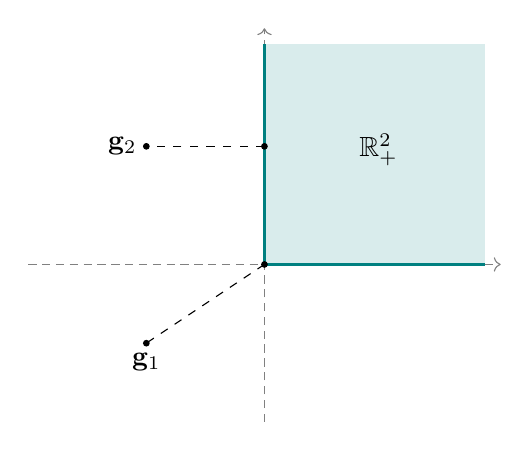
\begin{tikzpicture}
            \draw[densely dashed, gray][->] (0, -2) -- (0, 3);
            \draw[densely dashed, gray][->] (-3, 0) -- (3, 0);
            \path[fill=teal, fill opacity = 0.15] (0, 0) -- (0, 2.8) -- (2.8, 2.8) -- (2.8, 0) -- (0, 0) -- cycle;
            \draw[teal, line width=1pt] (0, 0) -- (0, 2.8);
            \draw[teal, line width=1pt] (0, 0) -- (2.8, 0);
            \filldraw (0, 0) circle (1pt);

            \begin{scope}
                \filldraw (-1.5, -1) circle (1pt);
                \draw[dashed] (0, 0) -- (-1.5, -1);
                \node at (-1.5, -1) [below]{$\mathbf{g}_1$};
            \end{scope}
            \begin{scope}
                \filldraw (-1.5, 1.5) circle (1pt);
                \filldraw (0, 1.5) circle (1pt);
                \draw[dashed] (0, 1.5) -- (-1.5, 1.5);
                \node at (-1.5, 1.5) [left]{$\mathbf{g}_2$};
            \end{scope}
            \node at (1.45, 1.45) {$\mathbb{R}^2_+$};
        \end{tikzpicture}
        \caption{}
    \end{subfigure}
    \caption{cone}
    \label{fig:cones}
\end{figure}

For an arbitrary cone, we first approximate it with polyhedral cones and then define the $k$th intrinsic volume as the limit
of the sequence formed by $k$th intrinsic volumes of the approximating sequence.

\begin{definition}
    Let $\mathcal{C} \subset \mathbb{R}^N$ be a closed convex cone.
    The statistical dimension $\delta (\mathcal{C})$ of the cone $\mathcal{C}$ is then defined as
    \[\delta(\mathcal{C}) = \sum_{k=0}^N k \nu_k (\mathcal{C}).\]
\end{definition}

\begin{example}
    Let $\mathcal{C} \subset \mathbb{R}^2 $ be a convex cone as shown in Fig.~\ref{fig:cones_a}.
    It has one zero-dimensional face (\{$\mathbf{0}$\}, the origin point), two one-dimensional faces (the two boundary rays)
    and one two-dimensional face (the cone itself).
    For the projection of vector $\mathbf{g}$ to be in the relative interior of a zero-dimensional face (which is also $\{\mathbf{0}\}$),
    the vector $\mathbf{g}$ has to be inside of the polar of $\mathcal{C}$, i.e., $\mathbf{g} \in \mathcal{C}^*$.
    The standard normal distribution is rotationally symmetric, so $\mathbb{P}\{ \mathbf{g} \in \mathcal{C}^*\} = \frac{\pi - \phi}{2\pi} $.
    Similarly, for $\op{proj}_{\mathca{C}} \mathbf{g}$ to lie inside $\mathcal{C}$, $\mathbf{g}$ itself must be inside of $\mathcal{C}$,
    which happens with probability $\frac{\phi}{2\pi}$.
    Finally, for one-dimensional faces we have the probability $\frac{1}{2}$.
    The statistical dimension can be easily calculated from the definition as
    \[ \delta (\mathcal{C}) = \frac{1}{2} + 2\frac{\phi}{2\pi} = \frac{\pi + 2\phi}{2\pi}.\]
\end{example}

\begin{example}
    The non-negative orthant $\mathbb{R}^N_+$ forms a polyhedral cone as an intersection of two half-spaces.
    It has one zero-dimensional face $\{\mathbf{0}\}$, $N$ one-dimensional faces of the form $\{0\}^k \times \mathbb{R}_+ \times \{0\}^{N-k-1}$
    for $k \in [\![ 0..N-1 ]\!]$, $\frac{N(N-1)}{2}$ two-dimensional faces of the form
    $\{0\}^k \times \mathbb{R}_+ \times \{0\}^j \times \mathbb{R}_+ \times \{0\}^{N-k-j-2}$ for
    $(k, j) \in  [\![ 0..N-2 ]\!]^2$ with $k+j = N-2$ and so on.
    In other words, $k$-dimensional faces only contain vectors with exactly $k$ non-zero components.
    Then $\op{proj}_{\mathbb{R}^N_+} \mathbf{g}$ lies in the relative interior of a $k$-dimensional face of $\mathbb{R}^N_+$
    if and only if $\mathbf{g}$ has exactly $k$ positive components, so
    \begin{equation*}
        {\nu_k(\mathbb{R}^N_+) = \mathbb{P}\{ \mathbf{g} \text{ has exactly } k \text{ positive components} \} }.
    \end{equation*}
    There are $\binom{N}{k}$ ways to ``choose'' which components will be positive.
    The probability of each component to be positive is $1/2$; the probability of it to be negative is also $1/2$.
    As they are independent from each other, we get the result
    \[{\nu_k(\mathbb{R}^N_+) = \frac{1}{2^N} \binom{N}{k}. \]
    The statistical dimension is then
    \[\delta (\mathbb{R}^N_+) = \frac{1}{2^N}\sum_{k=0}^N k \binom{N}{k} = \frac{N}{2^N} \sum_{k=0}^{N-1} \binom{N-1}{k} = \frac{N}{2}.\]
\end{example}

The topic of statistical dimension and conic intrinsic volumes is discussed in more detail in~\cite{statdim}.

\begin{theorem}
    Let $\x^* \in \mathbb{R}^N$ be a fixed vector and $p \in (0, 1)$.
    Suppose $\A \in M_{m \times N}(\mathbb{R})$ is a matrix with independent $\mathcal{N}(0,1)$-distributed entries and
    $\y = \A \x^*$.
    Then
    \begin{align*}
        & m \leq \delta(\mathcal{D}(\norm{\cdot}_1, \x^*)) - a_\eta \sqrt{N} \implies
        \mathbb{P}\{\x^* \text{ is the unique solution of \ref{eq:l1}}\} \leq \eta
        \\
        & m \geq \delta(\mathcal{D}(\norm{\cdot}_1, \x^*)) + a_\eta \sqrt{N} \implies
        \mathbb{P}\{\x^* \text{ is the unique solution of \ref{eq:l1}}\} \geq 1 - \eta,
    \end{align*}
    where $a_\eta = \sqrt{8 \log (4/\eta)}$.
    \label{th:lote}
\end{theorem}

\begin{figure}
    \begin{subfigure}{0.5\textwidth}
        \includegraphics[width=\linewidth]{pictures/compare_estimates1000}
    \end{subfigure}
    \begin{subfigure}{0.5\textwidth}
        \includegraphics[width=\linewidth]{pictures/compare_estimates10000}
    \end{subfigure}
    \caption{Comparison}
    \label{fig:compare}
\end{figure}

\section{Details of numerical experiments}

All of the plots shown here were done in Python.
At first, I tried to write my own implementation of the Chambolle-Pock algorithm (see~\cite{chambolle}),
but it wasn't fast enough for large numbers of tests, so I switched to \texttt{cvxpy} library.
For plots in figures \ref{fig:log} and \ref{fig:lote} I generated for each pair $(s, m)$ 10 random normal matrices and
10 $s$-sparse vectors $\x$ with non-zero components being either $1$ or $-1$.
Then corresponding vectors of measurements $\y$ were computed and the obtained problem was passed into the solver.
The result of the procedure was considered to be a success if the absolute error between $\x$ and the obtained solution
was less then $10^{-4}$.
Then the frequency of successful tests was calculated and ploted as a corresponding shade of gray, with white representing 100\%
success.

For the study of transition phase, the first major question was how to compute the statistical dimension of $\norm{\cdot}_1$.
Thankfully, the paper \cite{livingontheedge} provides us with the result below, that gives us tight bounds for the statistical dimension.

\begin{proposition}
    Let $\x \in \mathbb{R}^N$ be an $s$-sparse vector.
    Then the statistical dimension of the descent cone of the $l_1$ norm satisfies the inequality
    \begin{equation}
        \psi\left( \frac{s}{N} \right) - \frac{2}{\sqrt{sN}} \leq \frac{\delta(\mathcal{D}(\norm{\cdot}_1, \x))}{N}
        \leq \psi\left( \frac{s}{N} \right),
    \end{equation}
    where $\psi:[0,1] \rightarrow [0, 1]$ is defined as
    \begin{equation} \label{eq:inf}
        \psi(\rho) \coloneq \inf_{\tau \geq 0} \left[ \rho (1+\tau^2) +
        (1-\rho) \sqrt{\frac{2}{\pi}} \bigintssss_\tau^\infty  (u-\tau)^2  e^{-u^2/2}\mathrm{d}u \right].
    \end{equation}
\end{proposition}

The infimum in \ref{eq:inf} is achieved for the unique value of $\tau$ that solves the equation
\begin{equation} \label{eq:tau_eq}
    \sqrt{\frac{2}{\pi}}\bigintssss_{\tau}^{\infty} \left( \frac{u}{\tau} - 1 \right) e^{-u^2/2} \mathrm{d} u = \frac{\rho}{1 - \rho}.
\end{equation}
Integrals in \ref{eq:inf} and \ref{eq:tau_eq} can be simplified with the use of the error function (erf) to obtain more suitable
for computation quantities:
    \begin{gather}
        \sqrt{\frac{2}{\pi}}\tau^{-1}e^{-\tau^2/2} + \op{erf}\left( \frac{\tau}{\sqrt{2}} \right) - \frac{1}{1-\rho} = 0,
        \\
        \psi(\rho) \coloneq \inf_{\tau \geq 0} \left[ \rho (1+\tau^2) +
        (1-\rho) \left( \sqrt{\frac{2}{\pi}} \tau e^{-\tau^2/2} + (1+\tau^2)\left(\mathrm{erf}\left(\frac{\tau}{\sqrt{2}}\right) - 1\right) \right) \right].
    \end{gather}

Then these results were used to plot the curves corresponding to the statistical dimension and
bounds for the number of measurements from Theorem~\ref{th:lote}.

Another moment worth expanding on is how the green curve in Fig.~\ref{fig:compare} was obtained.
In the inequality (\ref{eq:log_improved}), probability depends on $m$, so to make this comparison fare,
we would have to choose a specific threshold for the probability and then compute the corresponding $m$, which is
exactly what was done.

Let $p$ be the desired minimal probability of the successful recovery.
Then we have an equation in terms of $m$:
\[ 1 - \exp \left( - \frac{1}{2} \left[\frac{m}{\sqrt{m+1}} - \sqrt {2s \log \frac{N}{s}+\frac{5}{4}s}\right]^2 \right) = p.\]
With some simple manipulations we get the solution of this equation:
\[ m = \frac{L^2 + L\sqrt{L^2 + 4}}{2}, \]
where $L = \sqrt{\log \frac{1}{(1-p)^2}} + \sqrt {2s \log \frac{N}{s}+\frac{5}{4}s}$.
\todo[inline]{Add link to github}

%\input{sections/conclusion}

    \nocite{*}
\printbibliography

\end{document}